\documentclass[aspectratio=169,professionalfonts]{beamer}

\usetheme{Madrid}
\usecolortheme{default}

\usepackage[T1]{fontenc}
\usepackage[utf8]{inputenc}
\usepackage{graphicx}
\usepackage{booktabs}
\usepackage{array}

\definecolor{CorbisNavy}{HTML}{102A43}
\definecolor{CorbisTeal}{HTML}{1F7A8C}
\definecolor{CorbisRust}{HTML}{B45309}
\definecolor{CorbisMist}{HTML}{F5F7FA}
\definecolor{CorbisSlate}{HTML}{334E68}

\setbeamercolor{structure}{fg=CorbisTeal}
\setbeamercolor{frametitle}{fg=white,bg=CorbisNavy}
\setbeamercolor{title}{fg=CorbisNavy}
\setbeamercolor{block title}{fg=white,bg=CorbisTeal}
\setbeamercolor{block body}{fg=black,bg=CorbisMist}
\setbeamercolor{alerted text}{fg=CorbisRust}
\setbeamercolor{item}{fg=CorbisTeal}

\setbeamertemplate{navigation symbols}{}
\setbeamertemplate{footline}[frame number]
\setbeamertemplate{blocks}[rounded][shadow=false]
\setlength{\columnsep}{1.4em}
\renewcommand{\arraystretch}{1.08}

\title{Corbis for Academic Research}
\subtitle{A beginner's guide to the Corbis tool\\and the Corbis Literature Starter Kit}
\author{}
\date{}

\begin{document}

\begin{frame}[plain,t]
\begin{columns}[c,onlytextwidth]
\column{0.47\textwidth}
{\usebeamerfont{title}\color{CorbisNavy}\LARGE\bfseries Corbis for\\Academic Research\par}
\vspace{0.6em}
{\large Getting started with Corbis and the Literature Starter Kit\par}
\vspace{1em}
\begin{block}{Who this is for}
Researchers who want to use AI assistants for literature reviews, idea screening, citation management, and a disciplined search trail.
\end{block}
\vspace{0.5em}
{\small
\textbf{Setup:} Claude Code, Codex, or Cursor with Corbis MCP.\\
\textbf{Goal:} Leave with a first workflow and first prompts to run.
}
\column{0.47\textwidth}

\includegraphics[width=\linewidth,height=0.62\textheight,keepaspectratio]{../images/corbis-landing-page.png}
\end{columns}
\end{frame}

\begin{frame}[t]{What Corbis Is}
\footnotesize
\begin{block}{Research-grade AI tools}
Corbis gives your AI assistant access to a curated academic corpus and returns results with citations you can inspect and verify.
\medskip

\scriptsize Start with \texttt{search\_papers}, \texttt{get\_paper\_details}, \texttt{top\_cited\_articles}, and \texttt{export\_citations}.
\end{block}
\begin{columns}[T,onlytextwidth]
\column{0.47\textwidth}
\begin{block}{What it provides via MCP}
\begin{itemize}
  \item Paper search, metadata, and citation export
  \item FRED macro data
  \item CRE market intelligence and dataset discovery
  \item Web search and deep research (select plans)
\end{itemize}
\end{block}
\column{0.47\textwidth}
\begin{exampleblock}{Why researchers should care}
\begin{itemize}
  \item Search the literature before making claims
  \item Trace where every piece of evidence came from
  \item Move from search to review to figures to writing in one repo
\end{itemize}
\end{exampleblock}
\end{columns}
\end{frame}

\begin{frame}[t]{Why This Repository Exists}
\small
\begin{block}{The problem}
AI assistants are fluent but undisciplined: they skip searches, hide provenance, and leave no research trail.
\end{block}
\begin{columns}[T,onlytextwidth]
\column{0.47\textwidth}
\begin{block}{What this kit adds}
\begin{itemize}
  \item 6 reusable research workflows
  \item Structured outputs in \texttt{notes/} and \texttt{output/}
  \item Automatic BibTeX export and LaTeX handoff
  \item Transparent search logging
\end{itemize}
\end{block}
\column{0.47\textwidth}
\begin{exampleblock}{What you gain}
\begin{itemize}
  \item Map a field in minutes, not days
  \item Screen ideas before committing weeks of work
  \item Keep a clean citation and writing pipeline
  \item Maintain a reproducible record of every search
\end{itemize}
\end{exampleblock}
\end{columns}
\end{frame}

\begin{frame}[t]{What a New User Needs}
\footnotesize
\begin{columns}[T,onlytextwidth]
\column{0.30\textwidth}
\begin{block}{Required}
\begin{itemize}
  \item A Corbis account
  \item A Corbis MCP API key
  \item An MCP-capable AI client
\end{itemize}
\end{block}
\column{0.30\textwidth}
\begin{block}{Recommended}
\begin{itemize}
  \item Claude Code for the smoothest slash-command flow
  \item Basic comfort with repo files
  \item Check citations before using them
\end{itemize}
\end{block}
\column{0.30\textwidth}
\begin{block}{Optional}
\begin{itemize}
  \item Python 3.10+ for figure generation
  \item LaTeX for manuscript drafting
  \item Codex or Cursor as alternative clients
\end{itemize}
\end{block}
\end{columns}
\vspace{0.6em}
\begin{alertblock}{Beginner rule}
Always search before asserting novelty, importance, or data availability.
\end{alertblock}
\end{frame}

\begin{frame}[t]{First-Time Setup in Claude Code}
\small
\begin{columns}[T,onlytextwidth]
\column{0.48\textwidth}
\begin{block}{Step 1: Create the key}
Open Corbis, go to \textbf{Settings > API Keys}, and create an MCP key. It starts with \texttt{corbis\_mcp\_} and is shown once.
\end{block}
\begin{block}{Step 2: Connect Claude Code}
{\scriptsize\ttfamily
claude mcp add corbis --transport http\\
https://www.corbis.ai/api/mcp/\\
universal?apikey=YOUR\_KEY
}
\end{block}
\begin{block}{Step 3: Work inside this repo}
Clone the starter kit, open it in Claude Code, and run your first workflow: \texttt{/lit-review [your topic]}.
\end{block}
\column{0.43\textwidth}
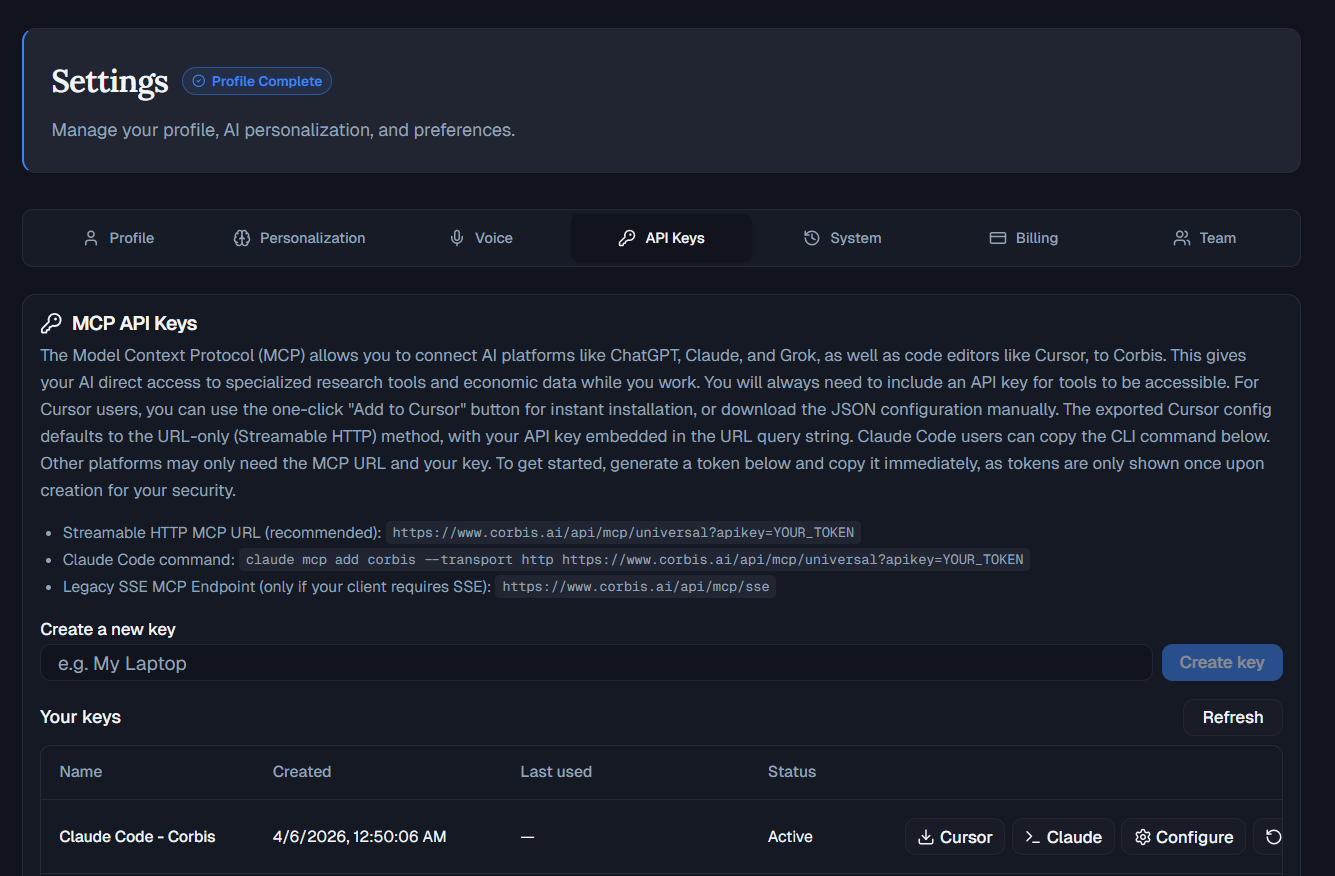
\includegraphics[width=\linewidth,height=0.58\textheight,keepaspectratio]{../images/corbis-api-keys.png}
\end{columns}
\end{frame}

\begin{frame}[t]{Other Client Paths}
\footnotesize
\begin{columns}[T,onlytextwidth]
\column{0.47\textwidth}
\begin{block}{Codex}
\begin{itemize}
  \item Add Corbis to your \texttt{config.toml} (global or project-level)
  \item Set the MCP server URL and a bearer token env var
  \item Export your key, restart Codex, verify with \texttt{codex mcp list}
  \item Full guide: \texttt{CORBIS\_MCP\_CODEX\_GUIDE.md}
\end{itemize}
\end{block}
\column{0.47\textwidth}
\begin{block}{Cursor}
\begin{itemize}
  \item Open \textbf{Settings > MCP Servers > Add}
  \item Name: \texttt{corbis}
  \item Paste the MCP endpoint URL with your API key
  \item Reload, then use workflow names as prompts
  \item Full guide: \texttt{CORBIS\_CURSOR\_PLUGIN.md}
\end{itemize}
\end{block}
\end{columns}
\vspace{0.5em}
\begin{exampleblock}{All clients, same tools}
Claude Code has the smoothest slash-command experience. Codex and Cursor use the same Corbis tools and the same workflow prompts from this repo.
\end{exampleblock}
\end{frame}

\begin{frame}[t]{Repository Map}
\scriptsize
\begin{tabular}{>{\raggedright\arraybackslash}p{0.27\textwidth} >{\raggedright\arraybackslash}p{0.65\textwidth}}
\toprule
\textbf{Path} & \textbf{Why a beginner should care} \\
\midrule
\texttt{.claude/commands/} & Slash-command wrappers (\texttt{/lit-review}, \texttt{/idea}, etc.) \\
\texttt{.claude/skills/} & Workflow definitions behind each command \\
\texttt{.claude/agents/} & Paper-reader prompt for deep reading of key PDFs \\
\texttt{notes/} & Lab notebook and dated research decisions \\
\texttt{output/} & Reviews, idea cards, figures, \texttt{paper\_set.json}, search log \\
\texttt{latex\_template/} & Clean article template (\texttt{natbib} + \texttt{plainnat}) \\
\texttt{utils/} & Python figure generator for \texttt{/lit-landscape} \\
\texttt{references/} & Writing norms and citation formatting \\
\bottomrule
\end{tabular}
\end{frame}

\begin{frame}[t]{How the Workflows Connect}
\footnotesize
\begin{columns}[T,onlytextwidth]
\column{0.45\textwidth}
\begin{block}{Shared files}
\begin{itemize}
  \item \texttt{output/paper\_set.json}: the canonical paper dataset reused across workflows
  \item \texttt{output/search\_log.md}: a transparent record of what the assistant actually searched
\end{itemize}
\end{block}
\begin{block}{The key idea}
Run one workflow to build a literature base. Later workflows reuse it instead of searching from scratch.
\end{block}
\column{0.45\textwidth}
\begin{exampleblock}{Typical chain}
\begin{enumerate}
  \item \texttt{/lit-review [topic]} builds the paper set.
  \item \texttt{/lit-landscape [topic]} turns that set into figures.
  \item \texttt{/brainstorm [topic]} proposes ideas against the same literature.
  \item \texttt{/idea [specific idea]} stress-tests one candidate.
\end{enumerate}
\end{exampleblock}
\end{columns}
\vspace{0.4em}
\begin{block}{Cross-client use}
\footnotesize In Claude Code these are slash commands. In Codex or Cursor, use the same names and examples as prompt templates.
\end{block}
\end{frame}

\begin{frame}[t]{Skill 1: \texttt{/lit-review}}
\small
\begin{columns}[T,onlytextwidth]
\column{0.39\textwidth}
\begin{block}{Use it when}
You need to understand a field before pitching, writing, or designing a project.
\end{block}
\begin{block}{Produces}
\begin{itemize}
  \item A synthesized review organized by theme
  \item A reading list of central papers
  \item BibTeX citations ready for your manuscript
  \item A reusable paper set for later workflows
\end{itemize}
\end{block}
\column{0.53\textwidth}
\begin{exampleblock}{Try it}
\texttt{/lit-review climate risk and commercial real estate}
\medskip
\begin{itemize}
  \item Good first move for a seminar paper or dissertation scan
  \item Clusters papers by theme, not just by keyword
  \item Leaves you with a reusable paper set for the next workflow
\end{itemize}
\end{exampleblock}
\end{columns}
\end{frame}

\begin{frame}[t]{Skill 2: \texttt{/lit-search}}
\small
\begin{columns}[T,onlytextwidth]
\column{0.39\textwidth}
\begin{block}{Use it when}
You already have a question or paper idea and need to locate the closest literature before claiming a contribution.
\end{block}
\begin{block}{Produces}
\begin{itemize}
  \item Closest 3--5 papers
  \item A draft contribution paragraph
  \item A related-literature outline
  \item BibTeX export for cited papers
\end{itemize}
\end{block}
\column{0.53\textwidth}
\begin{exampleblock}{Try it}
{\small\texttt{/lit-search Do bank branch closures reduce small business lending?}}
\medskip
\begin{itemize}
  \item Useful before a proposal meeting or referee response
  \item Searches by concentric rings: direct competitors, nearby methods, seminal work, recent papers
  \item Forces you to articulate how your paper differs
\end{itemize}
\end{exampleblock}
\end{columns}
\end{frame}

\begin{frame}[t]{Skill 3: \texttt{/brainstorm}}
\small
\begin{columns}[T,onlytextwidth]
\column{0.39\textwidth}
\begin{block}{Use it when}
You know the broad area but not which question is worth pursuing.
\end{block}
\begin{block}{Produces}
\begin{itemize}
  \item 10 ranked ideas from a wider candidate pool
  \item Expanded sketches for the top 3
  \item A recommendation for which idea to screen next
\end{itemize}
\end{block}
\column{0.53\textwidth}
\begin{exampleblock}{Try it}
{\small\texttt{/brainstorm behavioral biases in household mortgage decisions}}
\medskip
\begin{itemize}
  \item Good for early-stage dissertation exploration
  \item Applies multiple idea-generation lenses, then checks novelty against Corbis
  \item Kills weak ideas before you become attached to them
\end{itemize}
\end{exampleblock}
\end{columns}
\end{frame}

\begin{frame}[t]{Skill 4: \texttt{/idea}}
\small
\begin{columns}[T,onlytextwidth]
\column{0.39\textwidth}
\begin{block}{Use it when}
You have one concrete idea and want a hard-nosed screen, not encouragement.
\end{block}
\begin{block}{Produces}
\begin{itemize}
  \item An Idea Card with scoring and closest papers
  \item Novelty verification against Corbis
  \item Stress tests and essential hurdles
  \item A Go, Revise, or Kill verdict
\end{itemize}
\end{block}
\column{0.53\textwidth}
\begin{exampleblock}{Try it}
{\small\texttt{/idea Do zoning reforms lower rent growth by changing landlord expectations?}}
\medskip
\begin{itemize}
  \item Useful before spending weeks on data work
  \item Runs a desk-editor screen and three stress tests
  \item Identifies the hurdles you must clear and the exhibit you need
\end{itemize}
\end{exampleblock}
\end{columns}
\end{frame}

\begin{frame}[t]{Skill 5: \texttt{/verify-citations}}
\small
\begin{columns}[T,onlytextwidth]
\column{0.39\textwidth}
\begin{block}{Use it when}
You have a LaTeX manuscript and want to audit whether every citation is real, complete, and correctly matched.
\end{block}
\begin{block}{Produces}
\begin{itemize}
  \item A verification report
  \item Per-citation labels: OK, PARTIAL, MISMATCH, UNVERIFIED, or MISSING
  \item Checks against both the \texttt{.tex} and \texttt{.bib} files
\end{itemize}
\end{block}
\column{0.53\textwidth}
\begin{exampleblock}{Try it}
\texttt{/verify-citations}
\medskip
\begin{itemize}
  \item Final pass before circulating or submitting
  \item Catches stale BibTeX entries copied across projects
  \item Reduces embarrassing citation errors
\end{itemize}
\end{exampleblock}
\end{columns}
\end{frame}

\begin{frame}[t]{Skill 6: \texttt{/lit-landscape}}
\small
\begin{columns}[T,onlytextwidth]
\column{0.39\textwidth}
\begin{block}{Use it when}
You want figures that show trends, methods, and gaps in a literature.
\end{block}
\begin{block}{Produces}
\begin{itemize}
  \item Publication timelines and citation landmark charts
  \item Journal distributions and method evolution
  \item Thematic heatmaps and coverage gap maps
\end{itemize}
\end{block}
\column{0.53\textwidth}
\begin{exampleblock}{Try it}
{\small\texttt{/lit-landscape corporate governance and firm performance}}
\medskip
\begin{itemize}
  \item Useful for dissertations, review talks, or appendix figures
  \item Reuses \texttt{paper\_set.json} when available
  \item Requires Python: \texttt{pip install -r requirements.txt}
\end{itemize}
\end{exampleblock}
\end{columns}
\end{frame}

\begin{frame}[t]{Recommended Workflow}
\small
\begin{enumerate}
  \item \texttt{/lit-review [topic]} to learn the field and build the paper set
  \item \texttt{/brainstorm [topic]} to generate ideas, or \texttt{/lit-search [question]} to position an existing one
  \item \texttt{/idea [specific idea]} to screen before committing to heavy work
  \item \texttt{/lit-landscape [topic]} for visual evidence (talks, prospectus, appendix)
  \item Draft with \texttt{output/} files and the \texttt{latex\_template/}
  \item \texttt{/verify-citations} before circulating
\end{enumerate}
\vspace{0.7em}
\begin{alertblock}{The discipline}
Use Corbis to narrow the field. Use this repo to keep the search trail, outputs, and citations organized.
\end{alertblock}
\end{frame}

\begin{frame}[t]{Outputs and Research Hygiene}
\footnotesize
\begin{columns}[T,onlytextwidth]
\column{0.45\textwidth}
\begin{block}{What should stay in your repo}
\begin{itemize}
  \item \texttt{notes/lab\_notebook.md} for dated research decisions
  \item \texttt{output/*.md} for reviews, memos, and idea cards
  \item \texttt{output/paper\_set.json} and \texttt{output/search\_log.md}
  \item \texttt{.bib} exports plus the LaTeX manuscript files
\end{itemize}
\end{block}
\column{0.45\textwidth}
\begin{block}{Corbis extras outside the repo}
\centering
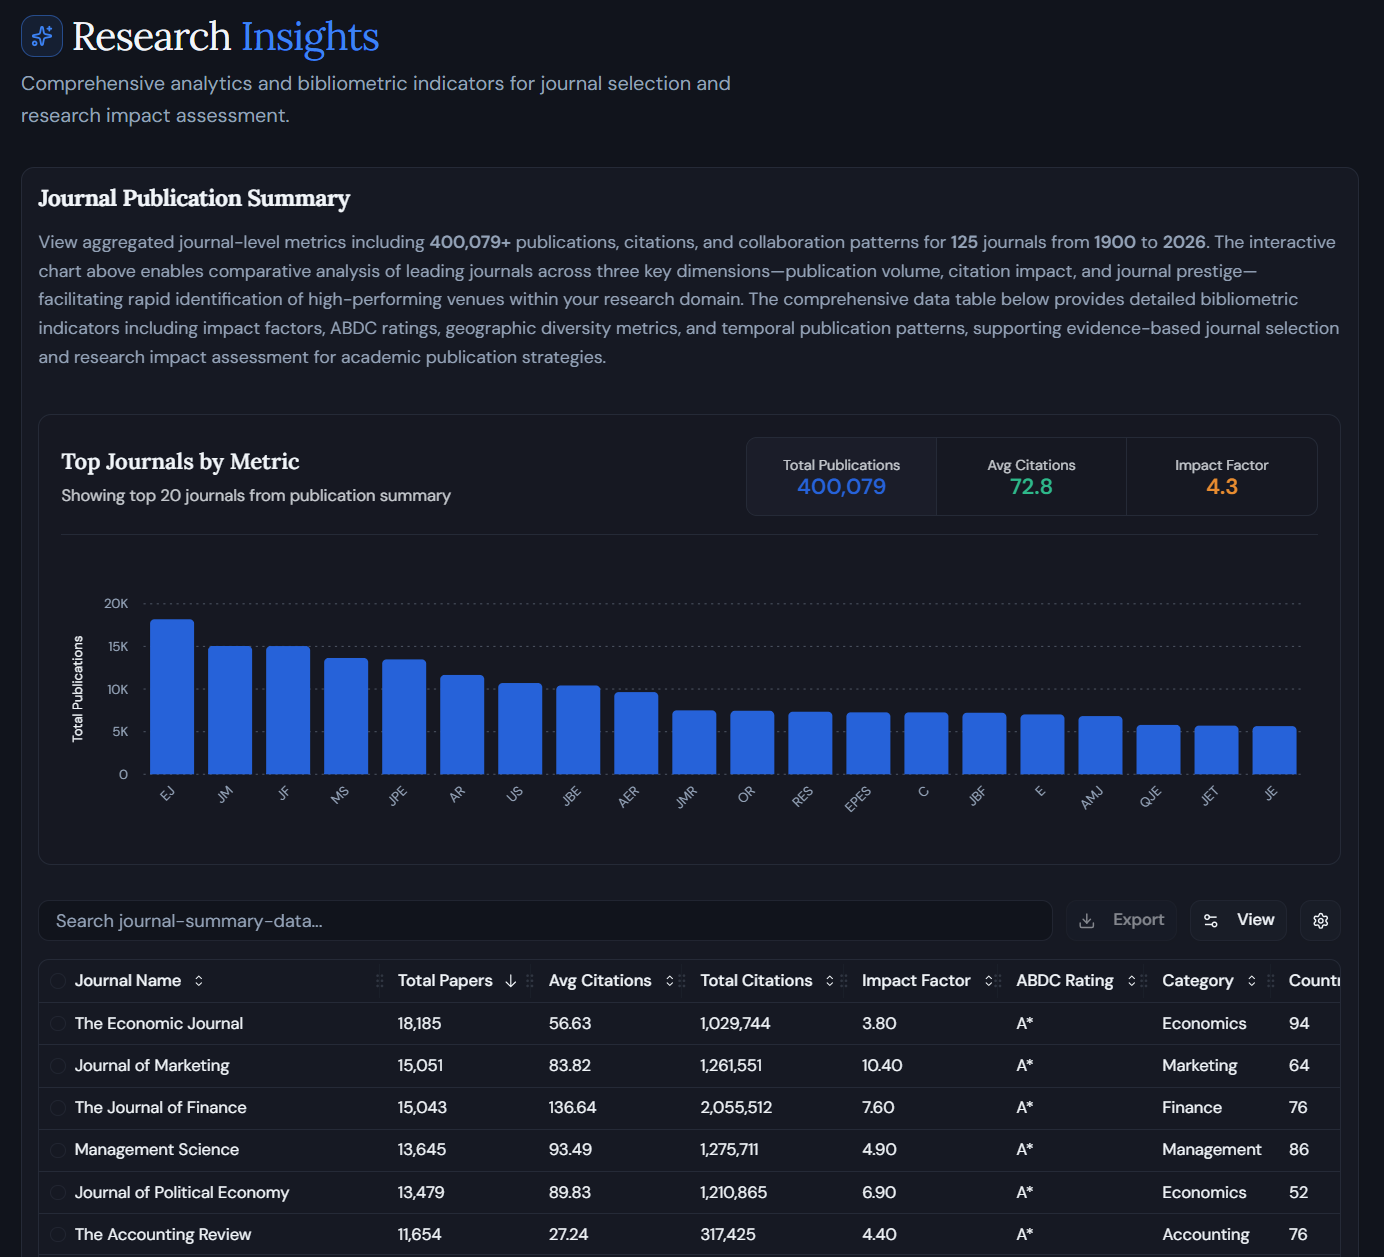
\includegraphics[width=0.46\linewidth,height=0.18\textheight,keepaspectratio]{../images/corbis-research-insights.png}
\hfill
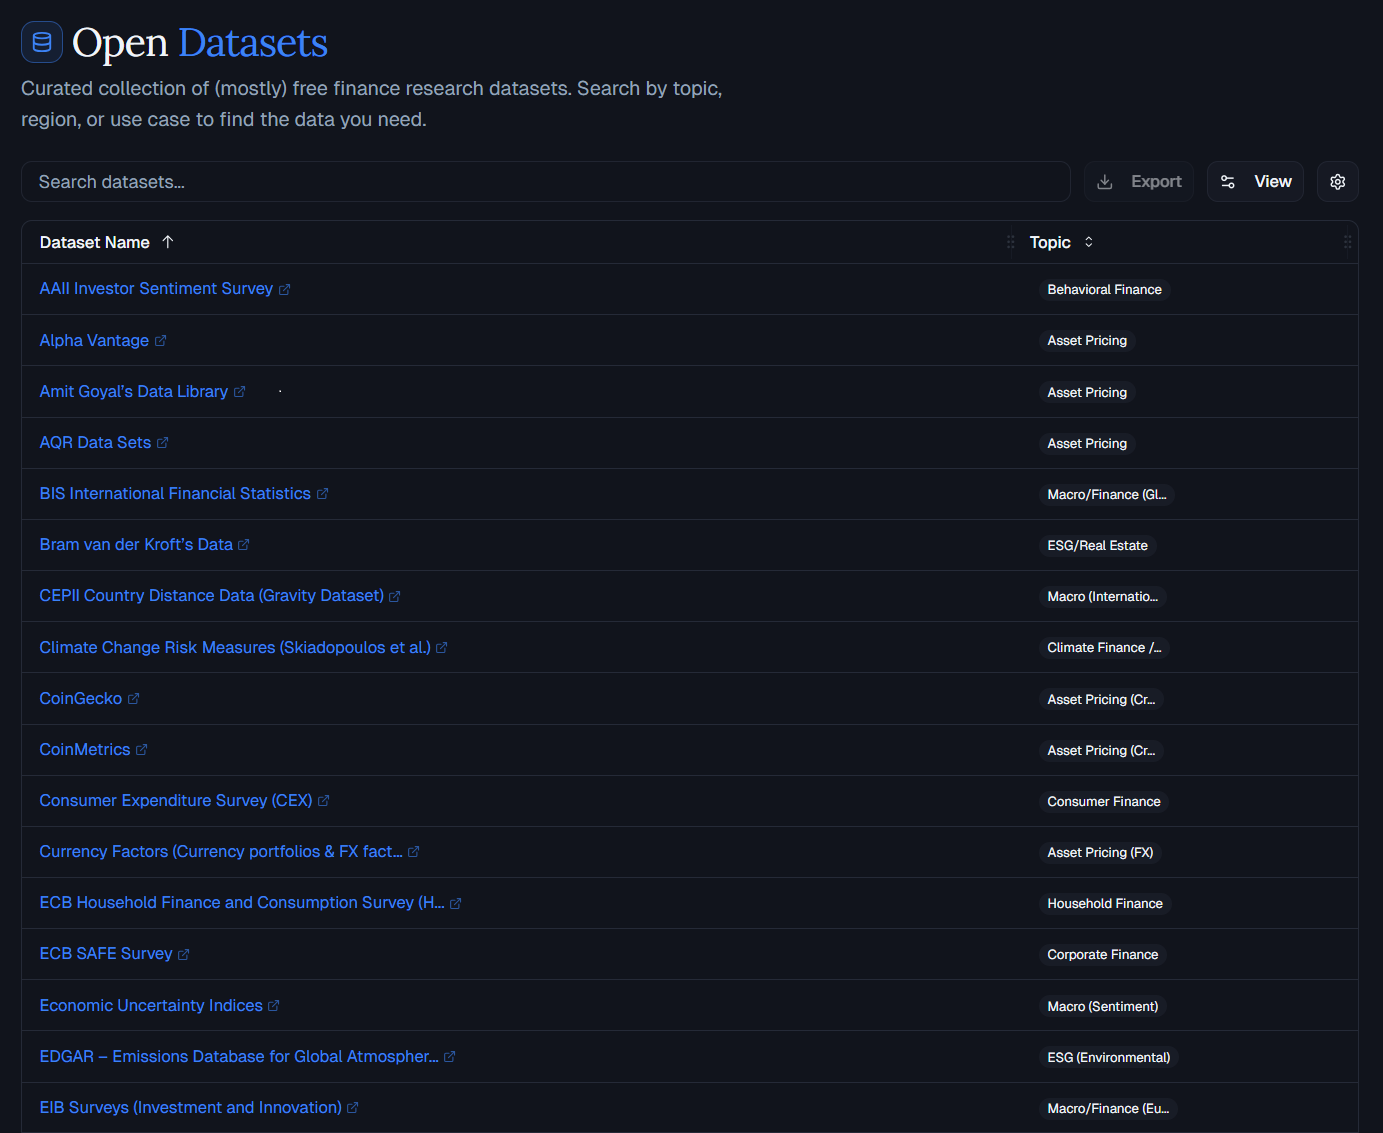
\includegraphics[width=0.46\linewidth,height=0.18\textheight,keepaspectratio]{../images/corbis-datasets.png}
\vspace{0.4em}

\raggedright
Research Insights gives journal-level corpus context. Open Datasets helps pair literature ideas with empirical data sources.
\end{block}
\end{columns}
\vspace{0.4em}
\begin{exampleblock}{Why this matters}
The repo gives you a search trail you can revisit, share, and reuse when the project evolves.
\end{exampleblock}
\end{frame}

\begin{frame}[t]{First Prompts to Try}
\footnotesize
\begin{block}{Start with these three}
\begin{enumerate}
  \item {\scriptsize\texttt{/lit-review climate risk and commercial real estate pricing}}
  \item {\scriptsize\texttt{/brainstorm behavioral biases in household mortgage decisions}}
  \item {\scriptsize\texttt{/idea Do bank branch closures reduce small business lending through relationship destruction?}}
\end{enumerate}
\end{block}
\begin{columns}[T,onlytextwidth]
\column{0.47\textwidth}
\begin{block}{Docs to keep nearby}
\begin{itemize}
  \item \texttt{README.md}
  \item \texttt{SKILLS\_USE\_GUIDE.md}
  \item \texttt{CORBIS\_MCP\_CODEX\_GUIDE.md}
  \item \texttt{CORBIS\_MCP\_TOOL\_REFERENCE.md}
\end{itemize}
\end{block}
\column{0.47\textwidth}
\begin{block}{Remember}
These workflows are not magic. They are a disciplined loop: search, synthesize, screen, document, verify.
\end{block}
\vspace{0.5em}
{\footnotesize
\href{https://www.corbis.ai}{corbis.ai} \hspace{1em}
\href{https://www.corbis.ai/docs}{www.corbis.ai/docs}
}
\end{columns}
\end{frame}

\end{document}
